\section{Introduction}
The past few years have witnessed the revolution of NLP methods with 
the advent of pretrained language models~(PLMs) such as 
\textsc{BERT}~\citep{DBLP:journals/corr/abs-1810-04805} and 
\textsc{RoBERTa}~\citep{DBLP:journals/corr/abs-1907-11692}. These
bi-directional Transformer~\citep{DBLP:journals/corr/VaswaniSPUJGKP17} 
encoders are first pretrained on vast amount of unlabeled text corpora and 
then fine-tuned on task-specific data, offering a surge of 
improvements on a wealth of downstream NLP tasks. Although this transfer learning paradigm has become the 
de-facto standard, we know very little about
\textit{what} and \textit{how much} 
knowledge embedded in PLMs actually contributes to the success. 
Notable endeavors toward this understanding focus on probing linguistic knowledge therein. They demonstrated that 
pretraining did impart useful linguistic abstraction about syntax and semantics into PLMs ~\citep{peters-etal-2018-dissecting,DBLP:journals/corr/abs-1901-05287,DBLP:journals/corr/abs-1905-06316}.


More recently, several works are presenting intriguing results examining 
 the relational knowledge within PLMs. Relational knowledge~\citep{speer-havasi-2012-representing,wikidata} is typically defined as describing the abstract relationship between a pair of concepts or entities, which is crucial for facilitating language understanding.
 \citet{Petroni2020} first posed the LAMA probe, 
 an English benchmark comprising multiple sets of prompts. Each prompt is a cloze-like sentence transformed from a relational knowledge triple:
 
 \noindent
 \textbf{Knowledge Triple: }\textit{$<$bus, HasA, ?$>$} \\
 \textbf{Object Label: }seats. \\
 \textbf{Sentence: }you are likely to find \underline{~~} in a bus.

 

By substituting  \underline{~~}  with a special [MASK] token and reusing the masked language modeling~(MLM) head, prompt-based relational knowledge probing provides an estimated lower bound of what PLMs know without training additional layer as in the previous linguistic probe. They showed that, even without grounded supervision, 
PLMs capture such relational knowledge at a level competitive to supervised alternatives. Subsequent works further showed that some specific prompts, acquired either through heuristical mining~\citep{DBLP:journals/corr/abs-1911-12543} or gradient-guided search~\citep{Shin2020}, can better trigger the models to correctly predict the missing object. 

Despite the mounting evidence for the existence of relational knowledge in PLMs, it remains unclear how such knowledge are represented internally. It hinders the utility of PLMs being extended to more structured tasks, such as knowledge base completion. In light of this, we raise the core question in this paper:
\textit{Can we disentangle PLMs into relation-specific knowledge models and take advantage of them in a more flexible way?}

We approach this question by first drawing inspiration from recent findings~\citep{DBLP:journals/corr/abs-2010-03648,DBLP:journals/corr/abs-2008-01064,inductivemlm}: \textit{the more cloze-like MLM pretraining simulates downstream task, the more successful the transfer will be.} For example, filling in \textit{like} or \textit{hate} into a cloze like \textit{I [MASK] this film, it's great.} provide a clear way in which the model can implicitly learn to perform sentiment classification. Similarly, we hypothesis that MLM pretraining on clozes expressing certain relation $r$ between masked word and remaining context would lead to good performance on knowledge probing that targets relation $r$. Instead of designing cloze instances resembling specific downstream tasks, we exploit such correlation conversely: \textit{the more successful the transfer is, the more cloze-like MLM pretraining simulates downstream tasks}.
Specifically, we propose \textbf{weakly supervised weights pruning}, 
an end-to-end differentiable procedure to search for different subnetworks within PLMs that target zero-shot knowledge probing of different relations. 

We show in experiment that it is possible to find subnetworks capable of representing grounded commonsense relations at non-trivial sparsity. \figref{fig:LAMA} exemplifies a cloze prompt where the identified subnetwork produces the valid answer \textit{seats} by attending to relevant 
context, i.e., bus,  while the full-scale \textsc{BERT} fails. We further investigate the possibility of  repurposing these subnetworks on various downstream tasks. Experimental results on commonsense knowledge base completion show that the identified subnetworks perform on par with or even better than strong supervised knowledge base completion methods. We also explore the usage of the subnetworks on multiple commonsense reasoning tasks and empirically find that, when combined properly, the subnetworks can outperform the original PLMs in both many-shot and zero-shot settings.

\begin{figure}[t]
	\centering
	\scalebox{1.0}{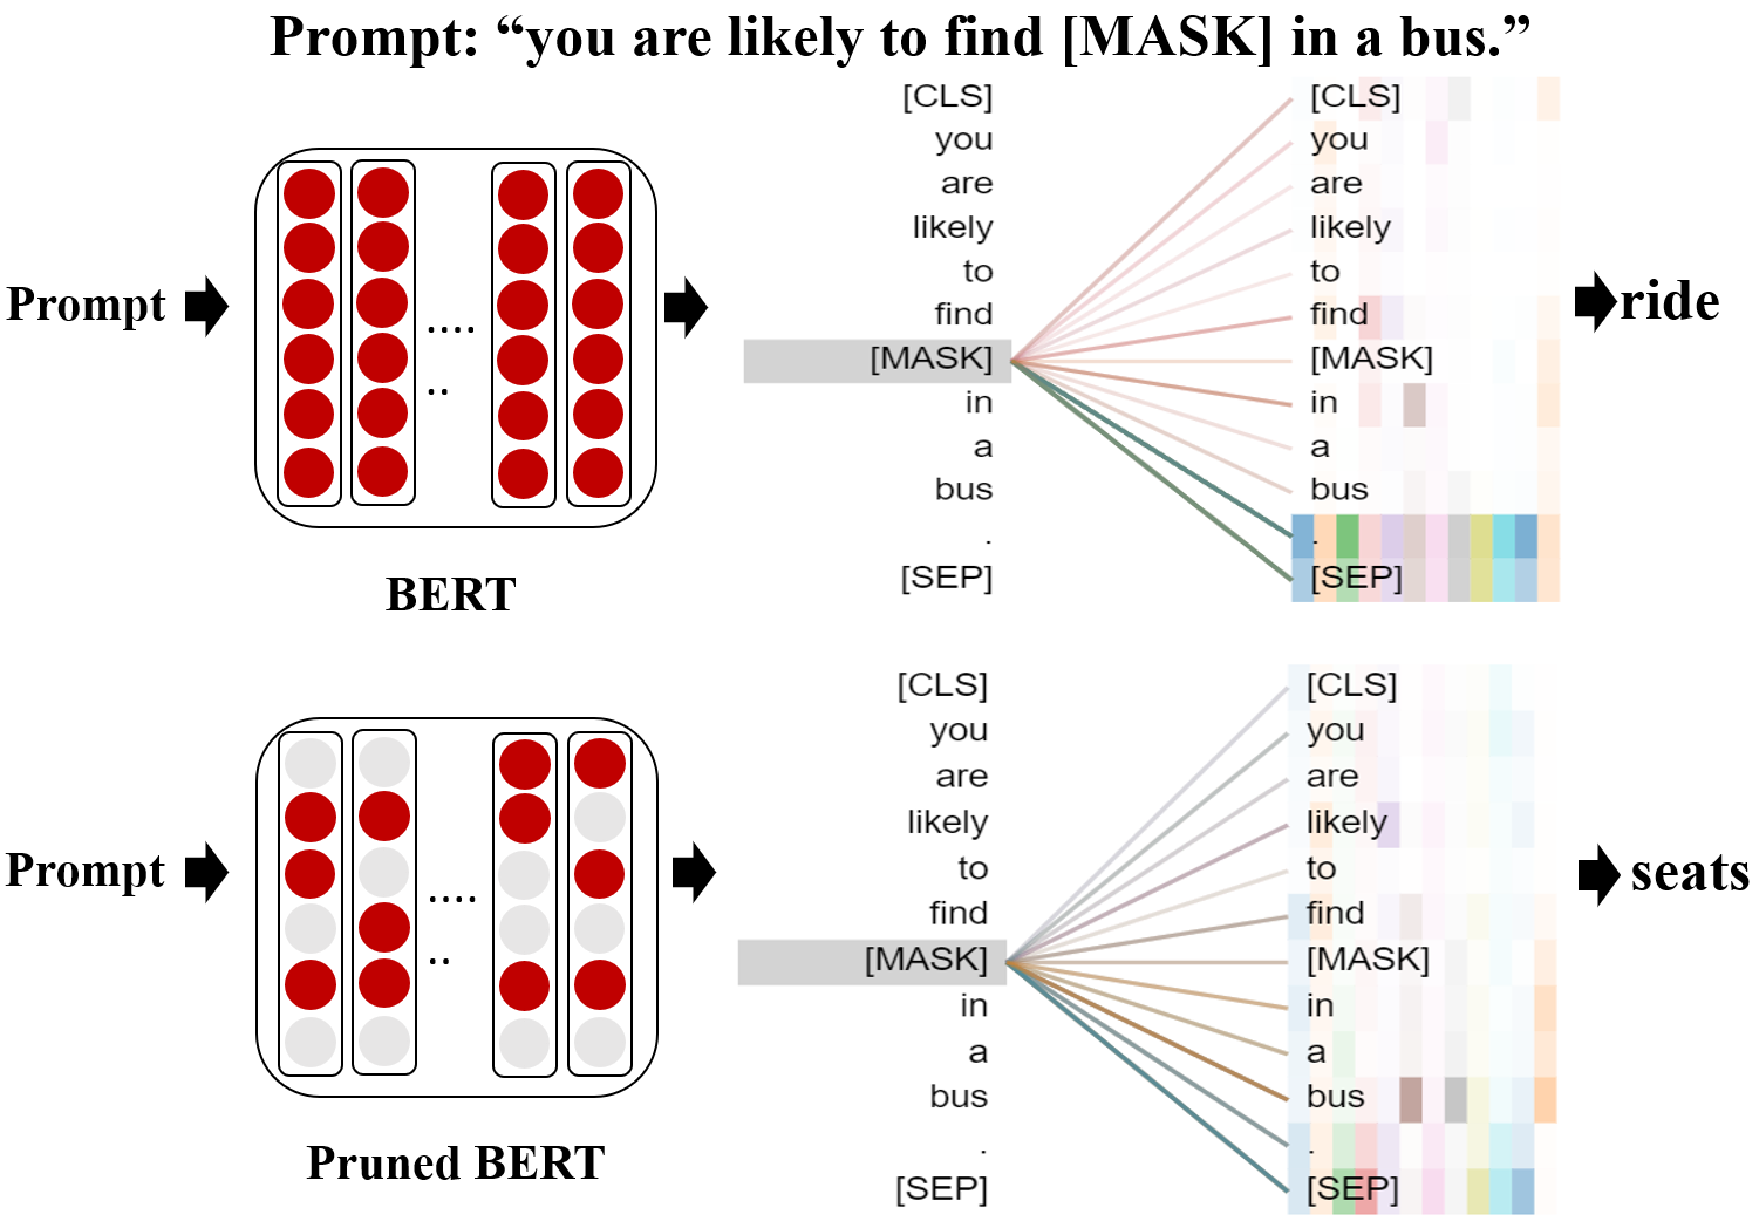
\includegraphics[width=1.0\columnwidth]{figure/intro.pdf}}
	\caption{Querying original/pruned \textsc{BERT-base} with prompts of relation \textit{HasA}. The color spectrum indicates the $12$ attention heads in the last layer~\citep{DBLP:journals/corr/abs-1904-02679}.} \label{fig:LAMA}
\end{figure}


In summary, our \textbf{contributions} include:
(i)~We present a novel way of eliciting relational knowledge hidden in PLMs from the perspective of network pruning~(\secref{sec:pruning}). (ii)~Grounding on a concept-centric relation schema, we show that the proposed pruning procedure successfully identified sparse subnetworks specializing in miscellaneous commonsense knowledge remarkably better than their full-scale counterparts~(\secref{sec:LAMA}). (iii)~We showcase the effectiveness of these subnetworks on commonsense knowledge base completion tasks~(\secref{sec:ckbc}) as well as a heuristic application on multiple commonsense reasoning tasks, gleaning insight on the transformation from language representation to knowledge representation.

We release code and all versions of our pruned PLMs at \url{https://anonymous.4open.science}.
